
\documentclass{article}
\usepackage[utf8]{inputenc}
\usepackage[a4paper, total={7in, 8in}]{geometry}
\usepackage{braket}
\usepackage{xcolor}
\usepackage{amsmath}
\usepackage{amssymb}
\usepackage{amsfonts}
\usepackage{graphicx}
\usepackage{svg}
\usepackage{media9}
\usepackage{float}
\usepackage{tikz}
% \usepackage{biblatex} %Imports biblatex package

\usepackage[
backend=biber,
style=alphabetic,
sorting=ynt
]{biblatex}

\addbibresource{sample.bib} %Import the bibliography file

\newcommand{\commentt}[1]{\textcolor{blue}{ \textbf{[COMMENT]} #1}}
\newcommand{\ctt}[1]{\commentt{#1}}
\newcommand{\prb}[1]{ \mathbf{Pr} \left[ {#1} \right]}
\newcommand{\onotation}[1]{\(\mathcal{O} \left( {#1}  \right) \)}
\newcommand{\ona}[1]{\onotation{#1}}
\newcommand{\PSI}{{\ket{\psi}}}
\newcommand{\LESn}{\ket{\psi_n}}
\newcommand{\LESa}{\ket{\phi_n}}
\newcommand{\LESs}{\frac{1}{\sqrt{n}}\sum_{i}{\ket{\left(0^{i}10^{n-i}\right)^{n}}}}
\newcommand{\Hn}{\mathcal{H}_{n}}
% \title{Understanding Quantum Computing}
% \author{David Ponarovsky}
% \date{July 2021}

\newcommand{\Ep}{\frac{1}{\sqrt{2^n}}\sum^{2^n}_{x}{ \ket{xx}}}
\newcommand{\HON}{\ket{\psi_{\text{honest}}}}
\usepackage{multicol}
% \usepackage{  }
\setlength{\columnsep}{0.6cm}


\begin{document}
    
\title{Weak qPCP (?)}
    
\maketitle
\begin{multicols*}{2}

% \paragraph{Definition.} \textit{we will say that an Hamiltonian set \( \mathcal{H} = \{ H_i \} \) is \textbf{\(\gamma\)-stable}  \ctt{CHANGE THE NAME}  if there is a constant \( \gamma > 0  \) such that for any state \( \PSI \) and the following enqulity holds:}
% \begin{equation*}
%     \begin{split}
%         \braket{\psi|\frac{1}{|\mathcal{H}|^2}\sum{H_{i}^{2}}|\psi} \le \gamma \cdot \braket{\psi|\frac{1}{|\mathcal{H}|}\sum{H_{i}}|\psi}
%     \end{split}
% \end{equation*}

\paragraph{Lemma.} \textit{ The promise problem \textbf{LH}\((k,a,b)\) such that \(a>\frac{9}{16} \) is \textbf{QMA}-complete. and there exist reduction that given a \textbf{LH}\((k,a,b)\) entity such that \(a < \frac{9}{16}\) returns \textbf{LH}\((k,a^\prime ,b^\prime)\) such that \textbf{(1)} \(a^\prime \ge \frac{9}{16}\), \textbf{(2)} the gap remains the same, \textbf{(3)} and the number of terms expand only by constant factor}.

The proof is trivial. 

\paragraph{Definition.} \textit{ Given Hamiltonian \( \mathcal{H} = \frac{1}{m}\sum_{i}{H_i}\) and a state \(\PSI\) we will define the \textbf{table form of} \( \PSI \) relative to \( \mathcal {H} \) to be the fowlling state over \(2n^2\) qubits: 
\begin{equation}
    \begin{split}
        & \text{Tableform}[\mathcal{H}, \PSI ] =
        \\ & \ \ \ \bigotimes\frac{1}{\sqrt{2}}\left(H_i\ket{\psi}\otimes \ket{\psi}+ \ket{\psi}\otimes H_j \ket{\psi}\right)
    \end{split}
\end{equation} We generalize that definition over set of states by  \(\text{Tableform}[\mathcal{H}, \Omega] = \{\text{Tableform}[\mathcal{H}, \PSI ] : \PSI \in \Omega \} \)}.

% \paragraph{Definition.} \textit{ We will say that state \(\PSI\) is an \textbf{\(l,k\)-almost copies product } (or just \textbf{\(lk\)-ACP}) if for any pair of two substring of \(\PSI\) at length \(l\) differ by at most \(2k\) qubits.} \ctt{another constraint should be append to that definition, \(\mathcal{H}\) define exactly the different.}     

\paragraph{Definition.} \textit{ Consider the \textbf{LH}\((k,a,b)\) and a space \(\Omega\) (not necessary vector space) such that the gap promise is valid only for states \(\in \Omega\). We will call to such problems \textbf{\(\Omega\)-weak promise local Hamiltonian} or just \textbf{\(\Omega\)-WLH}. Note, that every \textbf{LH}\((k,a,b)\) is also \textbf{\(\Omega\)-WLH} when \(\Omega\) is the whole space.}


\paragraph{Lemma.} \textit{Let \( \mathcal{H} = \frac{1}{m}\sum_{i}{w_{i}H_{i}}\) be a \(k\)-local Hamiltonian over \(n\) qubits with week promise over \(\Omega\), namely \textbf{\(\Omega\)-WLH}. Denote it's gap \(a-b = \Delta\). Then there is an explicit polynomial reduction (In the hardness sense) to an instance of \textbf{Tableform[\(\mathcal{H}, \Omega\)]-WLH} \(k\)-Hamiltonian over \(2\cdot n^2\) qubits which with promise \( (a^\prime, b^\prime) \) and a gap \(\Delta^\prime \ge 1.1\Delta\).}

\paragraph{Proof.} Consider a \(n \times n\) table such that each cell of the table holds \(2n\) qubits. And consider the Hamiltonian defined by
\begin{equation}
    \begin{split}
        \mathcal{H}^\prime = & \frac{1}{m^2}\sum_{ij}{ \overset{2\cdot i\cdot j-1}{\overbrace{I \otimes  I \otimes .. \otimes  I} } \otimes \\ & w_{i}w_{j}\left(H_{i} \otimes I   + I \otimes H_{j}  \right) \otimes   I \otimes  .. \otimes  I }       
    \end{split}
\end{equation}
Notice that each term act non trivaly on at most \(k\) qubits. In another hand, if there exist a state such that \( \bra{\psi}\mathcal{H}\ket{\psi} \ge a \) then the energy of the state \(\ket{\psi^\prime} = \bigotimes_{i,j}\frac{1}{\sqrt{2}}\left(H_i\ket{\psi}\otimes \ket{\psi}+ \ket{\psi}\otimes H_j \ket{\psi}\right)\) is also greater then \(a\). To see that let's analyze the contribution of the \(ij\)-term (up to \(w_{i}w_{j}\) factor): 

\begin{equation*}
    \begin{split}
        & \overset{2\cdot i\cdot j-1}{\overbrace{I \otimes  I \otimes .. \otimes  I} } \otimes \\ & \left(H_{i} \otimes I   + I \otimes H_{j}  \right) \otimes   I \otimes  .. \otimes  I \ket{\psi^\prime} = \\
        & ... \otimes \left(H_{i} \otimes I   + I \otimes H_{j}  \right)  \frac{1}{\sqrt{2}}\left(H_i\ket{\psi}\otimes \ket{\psi}+ \ket{\psi}\otimes H_j \ket{\psi}\right) \otimes .. =  \\ & 
        ... \otimes \frac{1}{\sqrt{2}} \left( 2H_{i}\ket{\psi}\otimes H_{j}\ket{\psi} +  H_{i}^{2}\ket{\psi} \otimes \ket{\psi} + \ket{\psi} \otimes H_{j}^{2}\ket{\psi} \right) \otimes ... = 
    \end{split}
\end{equation*}

% \begin{equation*}
%     \begin{split}
%          & ... \otimes \frac{1}{2} \left( 2H_{i}\ket{\psi}\otimes H_{j}\ket{\psi} +  H_{i}\ket{\psi} \otimes \ket{\psi} + \ket{\psi} \otimes H_{j}\ket{\psi} \right) \otimes ...
%     \end{split}
% \end{equation*}


Hence by projecting over \(\bra{\psi^\prime}\) it sufficent to look only on the following inner product: 

% \paragraph{} ddd
\begin{equation*}
    \begin{split}
        & \frac{1}{\sqrt{2}}\left(\bra{\psi}H_{i}\otimes \bra{\psi}+ \bra{\psi}\otimes  \bra{\psi} H_{j}\right) \\ &  \frac{1}{\sqrt{2}} \left( 2H_{i}\ket{\psi}\otimes H_{j}\ket{\psi} +  H_{i}\ket{\psi} \otimes \ket{\psi} + \ket{\psi} \otimes H_{j}\ket{\psi} \right) = \\ &
         \frac{1}{2} \left( 2\bra{\psi}H_{i}\ket{\psi}\cdot \bra{\psi}H_{j}\ket{\psi} + \bra{\psi}H_{i}\ket{\psi} \cdot \bra{\psi}\ket{\psi} + \\ & \ \   \bra{\psi}\ket{\psi} \cdot \bra{\psi}H_{j}\ket{\psi} \right)  
    \end{split}
\end{equation*}

Therefore:
\begin{equation*}
\begin{split}
    \Rightarrow \braket{\psi^\prime| \mathcal{H}^\prime | \psi^\prime } &= \frac{1}{2}\left(    \frac{1}{m}\sum_{i}\bra{\psi}w_{i}H_{i}\ket{\psi} \right)^2 + \\ & \frac{1}{2}\left( \frac{1}{m}\sum{w_{i}}  \right)\left( \sum_{i}\bra{\psi}w_{i}H_{i}\ket{\psi} \right)  
\end{split}    
\end{equation*}

It follows immediately that the gap over the \textit{table state} is bounded by \( a^\prime - b^\prime = \frac{1}{2}\left( a^2 - b^2  \right) + \frac{\sum{w_i}}{2m}\left(a-b\right) = \frac{1}{2} \left( a-b\right)\left(a + b\right)  = \left(\frac{a + b}{2} + \frac{\sum{w_i}}{2m}  \right)\Delta \). By assuming \(a > \frac{9}{16}\) and \(a -b > \frac{1}{poly(n)} \) we obtain that \( \Delta^{\prime} > 1.1\Delta \) \( \square\) 

\paragraph{NOTE.} If \(w_i < 0 \) we could replace the operator \(H_{i} \mapsto -H_{i}\) and it's still remain pauli operator.


\paragraph{Weak qPCP theorem.} \textit{ \(\textbf{QMA} < \textbf{qPCP}\left( \log n , 2^n)\right) \)} 
\paragraph{Proof.} Let \(\mathcal{H}\) be a local Hamiltonian. Let's repeat on the above construction in reqursive manner \( O(\log n) \) times, and denote the resoult by \(\mathcal{H}^{\star}\). Now if there exits, a state \( \PSI \) such that \( \braket{\psi|H|\psi} > a \) then it's clear that \( \text{Tableform}^{\log n}[\PSI] \) also has energy higher then \(a^{\prime}\) and in the same way if for every \(\PSI\) it holds that \( \braket{\psi|H|\psi} < b \) then the energy of every  \( \text{Tableform}^{\log n}[\PSI] \) will be less then \(b^{\prime}\). 

\begin{figure}[H]
  \centering
    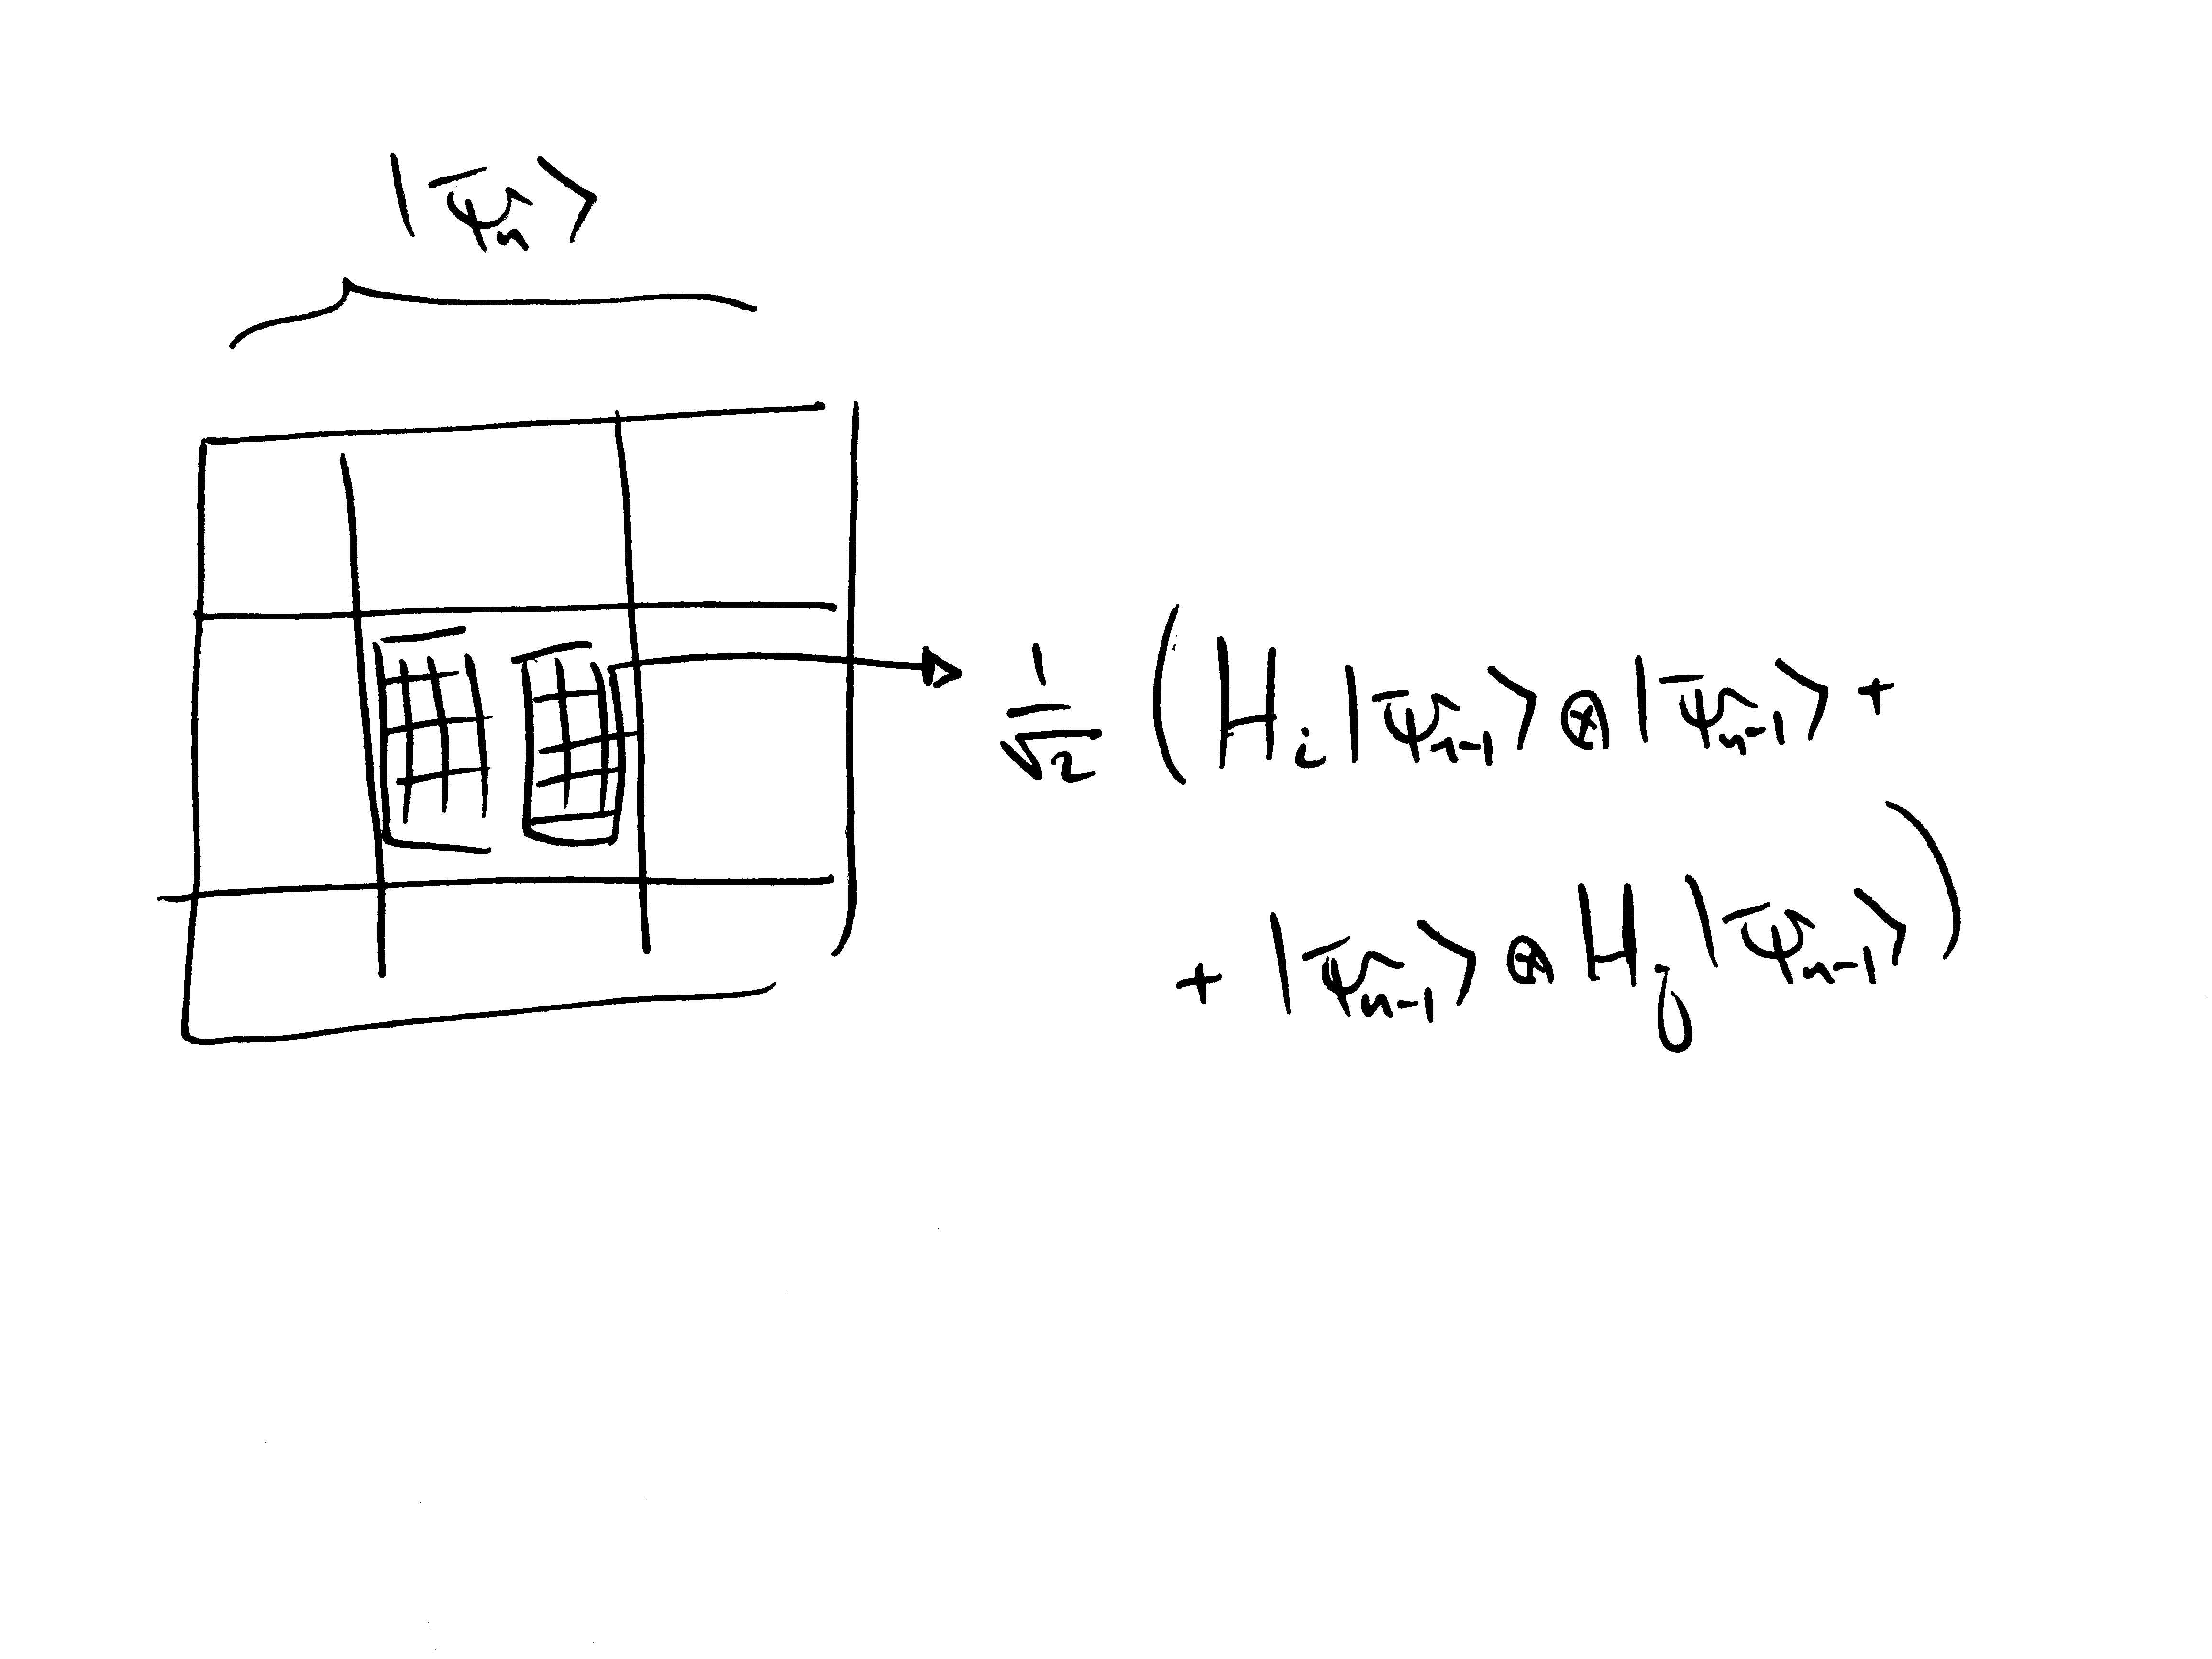
\includegraphics[width = 250pt]{outputt.jpg}
    \caption{The final tableform state, will be a table of \(\Theta(2^n)\) cells, each cell holds super position above two tensored tableforms at lower depth.}
    \label{fig:construction}
\end{figure}

\paragraph{Lemma.} \textit{Let \(J\) be cell at the lowest depth of the table. Then if \(\PSI\) is indeed a state in the reqursive tableform that were generated from \(\ket{\phi}\), then there is a set \( \left\{ H_1 , H_2 , H_3 .. H_{l \le \log n} \right\} \) such that:
\begin{equation*}
    \begin{split}
        \ket{J} &=  \frac{1}{2^{\frac{l}{2}}}\left(a_{0}I + a_{1}H_{1} + a_{2}H_{1}H_{0} + .. + a_{l}H_{l}..H_{2}H_{1}H_{0}\right)\ket{\phi} 
    \end{split}
\end{equation*} }


\paragraph{Proof.} By induction. base case: consider a single level construction. Then the table by definition is   \(\ket{\psi^\prime} = \bigotimes_{i,j}\frac{1}{\sqrt{2}}\left(H_i\ket{\psi}\otimes \ket{\psi}+ \ket{\psi}\otimes H_j \ket{\psi}\right)\). Let \(2\cdot(i,j)\) be an arbitrary cell.
\begin{equation*}
    \begin{split}
        &  \frac{1}{\sqrt{2}}\left( H_i \otimes I + I \otimes H_j \right) \ket{\psi}\otimes  \ket{\psi} \Rightarrow \\
        & \ket{J} = \left(\sum{\ket{n}\bra{n} \otimes I }\right)\frac{1}{\sqrt{2}}\left( H_i \otimes I + I \otimes H_j \right) \ket{\psi}\otimes  \ket{\psi} \\ 
        & 
    \end{split}
\end{equation*}
Assume the correctness of the Lemma for every \(n^\prime < n+1\), that is, every cell in the \(n\)-stage table can be expressed as linear combination of at most \(\log_n\). So we get that:
\begin{equation*}
    \begin{split}
        \frac{1}{2^{\frac{l}{2}}}\left(a_{0}I + a_{1}H_{1} + a_{2}H_{1}H_{0} + .. + a_{l}H_{l}..H_{2}H_{1}H_{0}\right)\ket{\phi} 
    \end{split}
\end{equation*}let's fix again a cell \((i,j)\) 

\paragraph{Lemma.} \textit{ Consider the product of \(\ket{\psi}\otimes\ket{\phi}\) there is a test which measure only \( O(1) \) qubits, accept with probability \(1\) if the states are equal and otherwise reject with probability \( p \).} 
\paragraph{Proof.} Perform the \textbf{SWAP} test on single arbitrary qubit. Assume that \( \ket{\psi} = \sum{w_i \ket{i}} \) and \( \ket{\phi} = \sum{w^{\prime}_i \ket{i}} \). Then the probability to measure \( \ket{0} \) is:
\begin{equation*}
\begin{split}
& \braket{0|0} = \frac{1}{2}\left(1 +  \frac{1}{n}\sum_{k}{ \bra{\psi , \phi}\textbf{SWAP}^{k}_{1} \ket{\psi, \phi}}   \right)  \\ 
& \bra{\psi , \phi}\textbf{SWAP}^{k}_{1} \ket{\psi, \phi} = \\& \sum{\braket{\psi^{i}_{1}..\phi^{j}_{k}..\psi^{i}_{n}\phi^{j}_{1}..\psi^{i}_{k}..\phi^{j}_{n}|\psi^{l}_{1}..\psi^{l}_{n}\phi^{m}_{1}..\phi^{m}_{n}}w_{i}w^{\prime}_{j}w_{l}w^{\prime}_{m}} = \\& \sum{\braket{\psi^{i}_{1}..\phi^{j}_{k}..\psi^{i}_{n}\phi^{j}_{1}..\psi^{i}_{k}..\phi^{j}_{n}|\psi^{l}_{1}..\psi^{l}_{n}\phi^{m}_{1}..\phi^{m}_{n}}w_{i}w^{\prime}_{j}w_{l}w^{\prime}_{m}}
\end{split}    
\end{equation*}

For each \(i,j\) pair there is a four pairs \(m,l\) such that the braket above is non zero, that because we can choose either \( l = m \) or that \(m = l \oplus e_{k} \). Let's compute each option separately:

\begin{equation*}
    \begin{split} 
        & \sum{\braket{\psi^{i}_{1}..\phi^{j}_{k}..\psi^{i}_{n}\phi^{j}_{1}..\psi^{i}_{k}..\phi^{j}_{n}|\psi^{i}_{1}..\psi^{i}_{n}\phi^{j}_{1}..\phi^{j}_{n}}w^{2}_{i}w^{\prime 2 }_{j}} = \\ 
        & \sum{\braket{\psi^{i}_{k}|\phi^{j}_{k}}^2w^{2}_{i}w^{\prime 2 }_{j}} = \sum_{i[k]=j[k]}{w^{2}_{i}w^{\prime 2 }_{j}} \Rightarrow 4 \sum_{i[k]=j[k]}{w^{2}_{i}w^{\prime 2 }_{j}} 
    \end{split}
\end{equation*}

We would expect that if the wights were disturbed uniformly then: 
\begin{equation*}
    \begin{split}
        \mathbb{E}\left[\sum_{i[k]=j[k]}{w^{2}_{i}w^{\prime 2 }_{j}}\right] &= \mathbb{E}\left[\sum_{i[k] \neq j[k]}{w^{2}_{i}w^{\prime 2 }_{j}}\right] \\
        \Rightarrow \mathbb{E}\left[\sum_{i[k]=j[k]}{w^{2}_{i}w^{\prime 2 }_{j}}\right] &= \frac{1}{2} \mathbb{E}\left[\sum_{ij}{w^{2}_{i}w^{\prime 2 }_{j}}\right] = \\ &= \frac{1}{2}\mathbb{E}\left[\sum_{i}{w^{2}_{i}}\right]\mathbb{E}\left[\sum_{j}{w^{\prime 2}_{j}}\right]\\ 
        &= \frac{1}{2}\braket{\psi|\psi}\braket{\phi|\phi}
    \end{split}
\end{equation*}

% \(\rightarrow\) If we could restrict our self only to tablesform states then we win. (we just need to apply the machinery of constant-gap after verify that the given state is indeed a tableform state). 

% Assume that we know what was the original form of \( \mathcal{H} \). Let \( \ket{\phi} \) be a state such that \(d\left( \ket{\phi},\textit{Tableform} \right) \ge d \cdot n \) that mean there is at least \(d\) leafs positions in the tree such the state which lay there.  Then we can a uncompute a single branch of the reqursive tree and by that "restore" the original state \( \PSI \). By choosing randomly pair of \(n\)-length slice of qubits (which mach to cells), we verify their uncompute by SWAP test. 
% So, let's attach to the beginning of the proof the classic encoding of the original Hamiltonian and we have done.      

% % \paragraph{Proof:} The proof it's treival, Let \(H\) be our original Hamiltonian and Consider the Hamiltonian which got by taking the weighted average of it with the identity. \(\square \)    



% \paragraph{Definition.}

% \paragraph{Definition.} \textit{ for a given state \(\ket{\psi} = \sum_{j}{\prod_{i}{\ket{x_{i}^{j}}}}\) we say that a unitary gate \(U\) \textbf{mixes} \(\ket{\psi}\) if there is bijection \( f\left(i,j\right) \mapsto \left(i^\prime,j^\prime\right)\) such that \(U\ket{\psi} = \sum_{j^\prime}{\prod_{i^\prime}{\ket{x_{i^\prime}^{j^\prime}}}}\). For a given set of states \(A\) and a gate \(U\) such that \(U\) mixes all the elements in \(A\) we will say that \(U\) mixes \(A\).}

% \paragraph{}
% Note that there is no exist a unitary gate which mix all the space \( \mathcal{H}^{*}\).  

% \paragraph{Definition.} \textit{ Let \(\Gamma\) be a constant integer, and \(\{I_{k}\}\) be a parttion over \(\mathbb{F}_{2}^{n}\) such \(\vert I_k \vert = \Gamma\). In addition consider a vector \(\phi_{0} \in \mathbb{F}_{2}^{n}\). A sate \(\ket{\psi}\) will called a \textbf{linear proof} if there are \( \left(\Gamma,\{I_k\}, \phi_0 \right)\) defined as above such: \begin{equation}
%     \ket{\psi} \propto \sum_{k}{\prod_{r \in I_{k}}{\ket{r,r \cdot \phi_{0}}}}
% \end{equation} till a normaliztion factor.}

% Notice that if a gate \(U\) mixes an linear proof \(\ket{\psi}\) then it will the turned state \(U\ket{\psi}\) is also a linear proof.    

% \paragraph{Definition.} \textit{An  \textbf{almost linear proof} will defined almost indentical to linear proof, except that now we replace the \(\psi_0\) parameter by asirea \(\{ \phi_{0}^{k} \}\) such that: \begin{equation}
%     \ket{\psi} \propto \sum_{k}{\prod_{r \in I_{k}}{\ket{r,r \cdot \phi_{0}^{k}}}}
% \end{equation} till a normaliztion factor.}

% Notice that by eaxmining only a single ket one can't distinguishing between an \textit{almost linear proof} and \textit{linear proof}. 

% \paragraph{Proposition.} \textit{Fix a constant integer \(\Gamma\), for every integer \(n\), Denote by \(A_n\) the set of all the almost linear proofs over \(n\) qubits  then there exists a unitary gate which mixes \(A_n\). }

% \textbf{Proof:} for \(n = \log\Gamma\). 

% \section{Property testing.} 
% The algorithm works as follow. An honest prover send the state:
% \begin{equation}
%     \HON = \sum_{k}{\prod_{r^{k}_{j} \in I_{k}}{\ket{r^{k}_{j},r^{k}_{j} \cdot \phi_{0}}}}
% \end{equation} 
% Then the verifier test by the classic weak-pcp check (measuring an ancila). If the given state pass the test then the verifier applies a generalize mixing and perform a second check.    
% \paragraph{Completeness} If \( \ket{\psi} =_{\sim I} \HON \) then it's clear that the first check pass with probability 1. Then in the second stage the mixed state is also \(=_{\sim I} \HON\) and therefore it will also pass the second check with probability 1.   
% \paragraph{Soundness} Suppose that 
% \begin{equation}
%      \vert\vert\braket{\psi|\psi_{\text{honest}}}\vert\vert^2 \le 1 - \varepsilon^{\star}
% \end{equation} 
% and denote by \(\varepsilon, \bar{\varepsilon}\) the sum of weight of the kets such that pass the the classic PCP test and don't accordingly. The first test fail to pass with probability at least \(\varepsilon\).   


% \paragraph{The Problem.} \(n\)-EPR pairs could be thought as resources in distributed computing with application in wide range of fields from the private key distribution till quantum teleportation. In this paper we consider an environment (ecosystem) in which one entity generate an highly entanglement state and sharing it between two other players who holds only a limited quantum ability. As the EPRS factory might be faulty we would like to verify that players indeed holds the correct state. And to ensure that the above indeed make sense we also require that only a minimal of EPRs will be measurement at the   verification process.

% Formally, we interest in verification protocol which compose from the following stages:
% \begin{enumerate}
%     \item \textbf{Initialization}, the factory initialize encoding of the EPR product and transmit to each player he's share.
%     \item \textbf{Verification}, the players are which limited only to single-qubit operations and measurements, and classical communication try to validate that they are indeed entanglement. 
%     \item \textbf{Decoding} if the players choose to accept the state then they could uncompute the encoding (restore the EPR product). 
% \end{enumerate}
% The idea behind the above form is that passing through a quantum channel is the most vulnerable stage in the total computation and therefore we are wishing to isolate it. Note that we are interesting in protocols in which the verification process pass for all the correct states and rejects with probability that proportional to the distance between the given state and the excepted one (in non faulty model).


% \ctt{delete} that it's success probability is function of both the rounds number it lasts and also the distance of the given state from the \(n\)-EPR state. Denote by \(\ket{\phi} \in \mathcal{H}^{poly(n)}\) the given state. And by 
% \begin{equation*}
% \begin{split}
%     \ket{\psi_n} = f \circ \bigleft( \frac{1}{\sqrt{2^n}}\sum^{2^n}_{x}{ \ket{xx}}  \bigright)
% \end{split}
% \end{equation*}
% for function \(f : \mathcal{H}^{poly(n)} \mapsto \mathcal{H}^{poly(n)}\). Denote by \(\mathcal{A}\) that algorithm, then there is a function \(g : \mathbb{N} \times (0,1) \rightarrow (0,1) \) :
% \begin{equation*}
%     \begin{split}
%         \prb{ \mathcal{A} \text{ reject} \ket{\phi}   } &\ge g\left( \text{time},d\left(\phi , \psi_{n} \right) \right)   
%     \end{split}
% \end{equation*}

% For example the algorithm which choose at each round a random pair of adjacent qubits, and then use them to play the Latin Square Game, fit for the setting above where \( f = \mathbf{I}\) and \( g(\text{rounds}) = \text{rounds}/n\). As far as we know there aren't results for protocols which their corresponded function \(g\) depends also on the distance. 



% \section{The Protocol.} 
% The verification protocol divide into two parts, first each party tests that he indeed holds a uniform superposition. We call that part \ctt{Thinks about a cool name}. Note that in the each party lab frame, the qubits state is an eigen state for X-Pauli errors, So if we have pass the phase error detection then it's only left to check that the state are don't have a "phase gap in the bits space". 
% \paragraph{Uniform superposition validation.}
% The factory wish to transmit the state \( \ket{\psi_n} = \Ep \). As the the left-\(n\) (right) qubits define the the left-\(x\) of \( \ket{\psi_n} \) kets then we could encode each of the halves separately  by generator \(G\) and initialize the state \( \frac{1}{\sqrt{2^n}}\sum^{2^n}_{x}{ \ket{G(x)G(x)}} \).

% Now after the transmission each party apply the error detection procedure. (And reject by probability proportional to the bit-flip distance between the state if a LTC code has been used). Note also that the encoded space is a uniform super position over the classical code words of \( \mathcal{C} \) and the phases are   By isomorphimsem we could assume that As the phase and the bit space are   It will be convenient to us      

% % \paragraph{Lemma I.} \textit{ Let \(\mathcal{C}\) be a Code with dimension \(O(1)\) fix+  }


% \paragraph{Proposition I.} \textit{Given a classic LTC  \(\mathcal{C}\) with \(\left[ n, \Theta(n), \Theta(n)  \right]\) parameters and a quantum LTC \(\mathcal{Q}\) with \(\left[ n, O(1), \Theta(n)  \right]_{q}\). Then one can construct a \(c^{3}\) quantum code}.

% \paragraph{Proof.} First, we will show explicitly the encoder gate. Let \(k\), \(m > k\) integers numbers, and \(J\) a subset of \(\left[m\right]\) such \(|J| = k\). Denote by \( \mathcal{T}_{J} : \mathcal{H}^{k+2m+k}_{2} \mapsto \mathcal{H}^{k+2m+k}_{2}  \) the quantum gate which first initializes \(m\) EPR pairs and then uses the \(J\) EPR's to transfer by teleportation the state defined by the first \(k\)-qubits to the last \(k\)-qubits with one exceptional change, we replace the measurements by cnot's. 

% Hence, the classic bit string which the parities transmitted through the channel is replaced by a the superposition over all the possible classic strings. 





% \paragraph{Proposition.} \ctt{Lemma.} For infinitely many \(n \in \mathbb{N}\) there is a constant depth circuit which verify uniform superposition with probability at least \(\alpha\) \ctt{complete}. 

% \textbf{Proof:} Assume that each ket of the state encoded by the LTC \( \mathcal{C} \), with generator matrix \(G\). And first apply the classic test over the state. 

% \begin{equation*}
%     \begin{split}
%         \prb{\text{ reject} \ket{\phi} } &= \bra{\cdot} \sum_{x \in [2^n] }{ \ket{x}\braket{x|\phi} \prb{\text{ reject x }  } } \\ 
%         &\ge \sum_{x \in [2^n] }{ ||\braket{x|\phi}||^{2} \frac{\omega}{m} d\left(x,\mathcal{C} \right) } \\ 
%         &= \sum_{x \notin \mathcal{C} }{ ||\braket{x|\phi}||^{2} \frac{\omega}{m} d\left(x,\mathcal{C} \right) } \\ 
%         &= \frac{\omega}{m} d\left(\phi,\mathcal{C} \right)
%     \end{split}
% \end{equation*}
% Hence if we pass the test defined by \( \mathcal{C} \) then till a \(Z\)-errors we are \(\delta\)-far from \( \ket{u_n} \). Diagonalize the state by H  the So it's sufficient to check that  

% \paragraph{Clocks syncorniztion.} from 

% \section{Different Points of View.}

% \paragraph{Locally Testable Codes.} Assume for the moment the existence of quantum locally testable code (qLTc). Then there is a local Hamiltonian that applying a random term of it over the state will measure energy above \( \gamma \) with probability greater then \( \frac{\omega}{m} d\left(\phi , \psi \right)\). Then the factory might pass the encoded state to the clients and. \ctt{...}  
% \paragraph{Alice-Bob Verification Game. } We could also think about a game in which a judge \(R\) try to verify that the parties \(A\) and \(B\) share an entangled state.  

% \paragraph{Definition. Leader Election State (LES).} For every \(n \in \mathbb{N} \) define the state \( \LESn \) to be  \begin{equation*}
%     \LESn = \LESs
% \end{equation*}  

% \paragraph{Proposition} There is a polynomial circuit that generate \(\LESn \). 

% \textbf{Proof.} Assume by induction correction for every \(n^{\prime} < n\). Then denote by \(U\) the gate which transform \(\ket{0}\) into the state \(\ket{\psi_{\frac{n}{2}}}\). \ctt{Handle the case where n is odd}.       
 
% \begin{figure}[H]
%   \centering
%     \includesvg[width = 250pt]{Gate.svg}
%     \caption{Comparison between}
%     \label{fig:average-sim-vs-model}
% \end{figure}
% The Depth of the circuit defined by recursive relation. 
% \begin{equation*}
% \begin{split}
%     \textbf{Depth}\left(n\right) &=\textbf{Depth}\left(\text{control-}U\right) + O\left(1\right) \\ & =\textbf{Depth}\left(U\right) + \textbf{Depth}(U^{\dagger}) + O\left(1\right) \\ &= 2\cdot\textbf{Depth}\left(\frac{n}{2}\right) + O\left(1\right) = O\left(n\right) \ \square
% \end{split}
% \end{equation*}
% \paragraph{}
% Then by the Theorem of Legal (guided local Hamiltonain is BQP-hard).\ctt{Spell the name and add citaion}. There exists a local Hamilton, such it's ground state has an overlap of at least \( \frac{1}{2} - \frac{1}{\text{poly}} \) with the history state. (the history state is the guided state (or the hint state) in he's reduction). From now on we will denote the Humiliation which corresponds to \( \LESn \) by \( \Hn \).  

% \paragraph{Assume} that the \textbf{NLTS} conjecture isn't correct. Then there is a trivial gate (with constant depth) which generate a state that approximate good as we wish the the ground state of \( \Hn \) and therefore also has \(\sim \frac{1}{2} \) overlap with the history state. \ctt{require a proof}.

% \paragraph{Proposition} For any \( n \in \mathbb{N}\) there is a trivial state which has \(\sim \frac{1}{2}\)-overlap with \( \LESn\). Denote it by \(\LESa\). \ctt{require a proof}.

% \paragraph{Proposition} There is a communication protocol which compute the \( \LESa \) in fixed number of rounds and every party communicate with a constant number of other parties. 

% \paragraph{Proposition} There is a asynchronous communication 1-resilient protocol which compute the \( \LESa \) in fixed number of rounds. Notice that probability to succeed doesn't depend on the enemy strategy.

% \textbf{Proof:} As every elementary quantum gate act over at most fixed number of qubits, then in every fixed depth/rounds circuit/protocol each gate could be feed with at most fixed number of non-honest inputs (\(f\)). Then we could divide each computation stage in our non-resilient protocol, which defined above, into groups of 
% \begin{equation*}
%     g = 4\left(f+1\right) + 1
% \end{equation*} parties and compute the gates via quantum Byzantine resilient protocol \ctt{the '\(+\)' inside the closures is critical}. Where passing \(\ket{0}^{\otimes n^{2}}\) (the input) is also considered as calculation step (gate), In our case \(f=1\). 

% For promising termination every honest party wait till he gets \(g - 1\) inputs, then he sets the last required message/pin to \(\ket{0}\) (\ctt{translate arbitrary error}), and continue forward to the error correction stage.

% \ctt{completing proof,  requires to handle the case when party should participate at the same time in two different groups. We should show that the depth overhand factor is a constant.}     

% % \paragraph{Proposition} \ctt{I don't sure that this proposal is true.} There is a asynchronous communication 1-resilient protocol which elects a leader, success with a.s probability and takes at most a fixed number of rounds.



% % \section{ Phase Estimation }
% % 
\paragraph{Introduction} Phase estimation is an example of a solvable problem in "constant" time classically (and quantumly). Yet, the less efficient quantum algorithm enables other algorithms to achieve quantum superiority by using superposition advantage.
The problem goes as follows, Let \(U \in \mathbb{M}_{2^n \times 2^n }(\mathbb{F})\) and \(v\) be a matrix and an eigenvector; what is the eigenvalue \(\lambda\) ? Classically, we answer it by calculating the quotient \( (Uv)_0/v_0 \) which done by \ctt{ add  time complexity of approximate linear operation with Boolean circuits over \(n\) bits.} The notations in the paper are attributed to Kitaev \cite{kitaev}.
\paragraph{quantum solution} Denote by \( U_{\oplus} \) the control-\(U\) gate. Let's look at the following composition of
operators \( H^{\dagger}U_{\oplus}H = HU_{\oplus}H \). Apply it over \( \ket{v}\ket{0} \) results : \begin{equation*} \begin{split}  H^{\dagger}U_{\oplus}H \ket{v}\ket{0} & = H^{\dagger}U_{\oplus} \frac{1}{\sqrt{2}}\left(\ket{v}\ket{0} + \ket{v}\ket{1} \right) \\ & = H^{\dagger} \frac{1}{\sqrt{2}}\left(\ket{v}\ket{0} + \lambda\ket{v}\ket{1} \right) \\ & = \frac{1}{2}\left(\ket{v}\left(\ket{0}+\ket{1}\right)+\lambda\ket{v}\left(\ket{0}-\ket{1}\right)\right) \\ & = \frac{1}{2}\left(1+\lambda\right)\ket{v}\ket{0} + \frac{1}{2}\left(1-\lambda\right)\ket{v}\ket{1} \end{split}\end{equation*}  measurement the \textit{ancila} qubit yields \( \ket{0} \) with probability \( \prb{ \ket{a} = \ket{0} }  = \big| \frac{ 1 + \lambda}{2} \big|^2 \sim \frac{1}{2}\left( 1 + \cos (\theta) \right)  \). Where \( \theta\) denote the projection angle of the results vector. And using Chernoff inequality bound, \[ \prb{ \big| \frac{1}{k}\sum_{i}^{k}{x_i} - \mathbf{E}[x] \big| \ge \varepsilon} \le 2exp\left( -\frac{k\varepsilon^2}{2} \right) \] It is enough to repeat the calculation \ona{ \frac{1}{\varepsilon^2}  \log\left(\frac{1}{\delta}\right) } to ensure that with probability at least \( \delta \) we will estimate the eigenvalue with error less than \( \frac{\varepsilon}{2} \). Note, that  \( \varepsilon \)  isn't  depend on the dimension of \( U \), neither \( \delta \).
In addition suppose, that we have an access to the circuit \( U^{2^t} \), then we could estimate \( \lambda \) with an error of \( 2^{-t} \) by using take sqrt \( t\) times,  \[ \tilde{\lambda}_{2^{t-1}} \leftarrow \sqrt{\tilde{\lambda}_{2^t} + \varepsilon }\le  \sqrt{\tilde{\lambda}_{2^t}} + \frac{1}{2}\varepsilon \]Hence achieving precision of \( 2^{-m} \) requires an order of \ona{ m\log(m)} operations \ctt{Fix that sentence, the operations are required for calculating the \(U^{2^t} \) gate } .      
\paragraph{Factoring} At first sight, It is hard to notice if the quantum approach holds any advantage at all. Now we will introduce an application which wins the best known classical algorithms, for integers factoring.
Consider the natural number \( 1 < N  \le 2^n \) at length \( n \) bits, with \(k\) prime factors \( N = p_{1}^{e_1}p_{2}^{e_2}p_{2}^{e_2}...p_{k}^{e_k} \). The general method for decompose number is to find \(x\) such that \( x^2 \equiv 1 \left( mod \ N \right) \) and  \( x\neq \pm 1  \left( mod \ N \right) \). Since \[0 = x^2 - 1 = \left(x-1\right)\left(x+1\right) \Rightarrow x+1 \ | \  N \] At least one of \( x \pm 1 \) is less than \( \sqrt{N} \)  then given efficient method to find such \(x\)'s we can complete the task by \ona{\log\log N}  recursive iterations. Unfortunately (or luckily), the best such classically subroutines require super polynomial time (note that the problem isn't (probably) \textbf{NP}-complete since there are (classically) sub-exponential solutions).
\commentt{ Insert definition of the ismorphisem \( \varphi : \mathbb{Z}_N \mapsto  \mathbb{Z}^{*}_{N} \ \)    }
\paragraph{Definition} For \( \vec{a} \in \mathbb{Z}^{*}_{N} \) denote by the \(r\) the minimal number such that \( \vec{a}^{r} \equiv 1 \), then we call for \(r\) the order of \(\vec{a} \). 
\paragraph{Lemma} For uniformly chosen \( a \in \mathbb{Z}_N \) the rank of \( \varphi(a) \in \mathbb{Z}^{*}_{N} \) is even with high probability, greater then \( \ge 1 - 2^{-n+1}  \). 
In other words, \( b = a^\frac{r}{2} \) is integer which satisfy the equation: \(b ^2 = 1\).   
\paragraph{quantum solution} Choose uniformly \( a \in \mathbb{Z}_N \), and construct the gates \( U_{a}, U_{a}^{2} ... U_{a}^{2^t}  \) \[ U_{a}\ket{x} = \begin{cases} \ket{ax \ mod N} & (x,N)=1 \\ \ket{x} & else  \end{cases} \] 
let \( w = e^{i\frac{2\pi}{r}}\)  consider the Fourier base \[ \ket{\psi_k} = \frac{1}{\sqrt{r}}\left( \ket{1} + w^{-k}\ket{a} + w^{-2k}\ket{a^2} ...  + w^{-(r-1)k}\ket{a^{r-1}}\right) \] then \( U_{a} \) applying \( U_a \) over \( \ket{\psi_k} \) yields: \[ \begin{split}
U_{a}\ket{\psi_k} & = \frac{1}{\sqrt{r}}U_{a}\left( \ket{1} + w^{-k}\ket{a} + w^{-2k}\ket{a^2} ...  + w^{-(r-1)k}\ket{a^{r-1}}\right)  \\ & = 
\frac{1}{\sqrt{r}}\left( U_{a}\ket{1} + w^{-k}U_{a}\ket{a} + w^{-2k}U_{a}\ket{a^2} ...  + w^{-(r-1)k}U_{a}\ket{a^{r-1}}\right) \\ & = \frac{1}{\sqrt{r}}\left( \ket{a} + w^{-k}\ket{a^2} + w^{-2k}\ket{a^3} ...  + w^{-(r-1)k}\ket{1}\right)\\ & = w^{k}\ket{\psi_k}  \end{split} \] That is, \( \ket{\psi_k} \) is an eigenvector with eigenvalue \( w^{k}=e^{i\frac{2\pi k}{r}} \). Note that, if we knew the base \( \ket{\psi_k} \), we could estimate the phase classically in \ona{ \mathbf{Poly} (r)  } time, and then extract the order of \(a\). The problem is that we do not know. Here quantum mechanics proves it's \textbf{Superiority}, let's look of \( \ket{1} \) state: \[ \braket{\psi_{k}|1} = \frac{1}{\sqrt{r}} \]Therefore The presentation of  \( \ket{1} \) in the Fourier base is \[ \ket{1} = \sum_{k}^{r} {\braket{\psi_{k}|1}\ket{\psi_{k}}} = \frac{1}{\sqrt{r}}\sum_{k}^{r} {\ket{\psi_{k}}} \]Therefore \( \ket{1} \) is the uniform weighted superposition of all \( \ket{\psi_k} \). So we will execute the circuit over \( \ket{1} \) then the after the measurement we will estimate a phase of \( \frac{k}{r} \) for arbitrary \(k\). for finding the most significant bit of \(r\) we could look in binary search; we will sample a \(T\) results and ask if at least \(\frac{1}{2}\) of them are beneath \(2^j\), if the answer is positive then \(r\) \le \(2^{j+1}\) with high probability, else. we will check \(2^{j+1} \).  \commentt{Improve the language. }      



\paragraph{Definition Span Program.} \cite{algo} A span program, \( P = \left(H, \mathcal{U} ,\tau,A\right) \) on \( \{0,1\}^N \) is made up of \textbf{(1)} finite-dimensional inner product space \( H = H_1 \oplus H_2 .... \oplus H_N \), and \( \{ H_{j,b} \subset  H_j \}_{j\in [N], b\in \{0,1\}} \) such that \( H_{j,0} + H_{j,1} = H_j \), \textbf{(2)} a vector space \( \mathcal{U} \). \textbf{(3)} a non-zero target vector \( \tau \in \mathcal{U} \), and \textbf{(4)} a linear operator \( A : H \Rightarrow \mathcal{U} \). for every string \( x \in \{0,1\}^N \) we associate the subspace \( H(x):= H_{1,x_1}\oplus ... \oplus H_{N,x_N} \) and an operator \( A(x):= A\Pi_{H(x)} \). 

\paragraph{Definition (Positive and Negative Witness}. Let \(P\) be a span porgram on \( \{0,1\}^N \) and let x be a string \( x \in \{0,1\}^N \). Then we call \( \ket{w} \) a positive witness for \(x\) in \( P\) if \( \ket{w} \in H(x) \) , and \( A\ket{w}=\tau \). We define the positive witness size of \(x\) as: \[ w_{+}(x,P) = w_{+}(x) = \min{\{ \norm{\ket{w}}^2: \ket{w} \ is  \ a \ positive \  witness \}} \] if there exists a positive witness  for \(x\) and \( w_{+} (x) =\infty \) otherwise.
Let \((\mathcal{L},\mathbb{R})\) denote the set of linear maps from \( \mathcal{U} \) to \( \mathbb{R} \). We call a linear map \( w \in (\mathcal{L},\mathbb{R})\) a negative witness for \(x\) in \(P\) if \( wA\Pi_{H(x)}=0\) and \( w\tau =1 \). We define the negative witness size of \(x\) as: \[ w_{-}(x,P) = w_{-}(x) = \min{\{ \norm{wA}^2: w \ is  \ a \ negative \  witness \}} \] if there exist one, and  \(\infty \) otherwise. If \( w_{+}(x) \) is finite, we say that \(x\) is positive, and if \( w_{_}(x) \) is finite, we say that \(x\) is negative.
For function \( f : X \rightarrow \{ 0,1\} \), with \( X \subset \{0,1\}^N \), we say \(P\) decides \(f\) if \( f^{-1}(0)\subset P_0 \) and \( f^{-1}(1) \subset P_1 \). (with high probability), given access to the input \(x \in X\) via queries of the form \( \mathcal{O}_x : \ket{i,b}\mapsto \ket{i,b\oplus x_i}\).
\paragraph{ Theorem }. Let \( \mathcal{U}(P,x) = \left( 2\Pi_{\ker A } - I\right)\left(2\Pi_{H(x)} - I \right)\). Fix \( X\subset \{0,1\}^N \) and \( f:X\rightarrow \{0,1\} \) and let \(P\) be a span program on \( \{0,1\}^N \) that decides \(f\). Let \( W_{+}(f,P) = \max_{x\in f^{-1} (1)}w_{+}(x,P) \) and \(W_{-}(f,P) = \max_{x\in f^{-1} (0)}w_{-}(x,P) \). Then there is a bounded error quantum algorithm that decides \(f\) by making \ona{\sqrt{W_{+}(f,P)W_{-}(f,P)}} calls to \( \mathcal{U}(P,x) \). \commentt{Add proof for that theorem.} 

\paragraph{st-Connectivity Span Program.} Consider the graph \(G\) with some implicit weighting function \(c\). Let define the \(P_G\) span program by \textbf{(1)} \( \forall i \in \left[N\right], b\in \left\{0,1\right\} : H_{i,b} = span\left\{ \ket{e} : e \in \vec{E_{i,b}} \right\} \),  \textbf{(2)} \( \mathcal{U} = span\left\{ \ket{v} : v \in V(G) \right\} \), \textbf{(3)} \( \tau = \ket{s} - \ket{t} \)  and for all edge \(e\), \textbf{(4)} \( A\ket{uvl}= \sqrt{c\left(u,v,l)\right) } \left( \ket{u} - \ket{v} \right) \).   It can shown that \(x\) is a positive input for \(P_G\) if and only if \( G(x) \) is st-connected, and in particular \( w_{+} (x,P_G) = \frac{1}{2}R_{s,t}(G(x)) \).

\newcommand{\V}{  V\left( G \right) }
\newcommand{\E}{  \vec{E}\left( G \right) }
\newcommand{\Projx}[2]{ \sqrt{c\left(u,v,l\right) } \left( #1 - #2 \right) }
\newcommand{\Proj}[]{ \Projx{\ket{u}}{ \ket{v}} }
\newcommand{\Vw}[1]{\mathcal{V}_w \left(#1\right)}
\newcommand{\tu}{\left(u,v,l\right)}

\newcommand{\Pot}[]{\mathcal{V} \left(v\right) \bra{v}}

\paragraph{Theorem.} Let \(P_G\) be the span program which defined above. Then for any \( x \in \{0,1\}^N \) \[ w_{-}\left(x,P_G\right) = 2C_{s,t}\left(G\left(x\right)\right) \]. 
\paragraph{Proof.} Given a unit st-potential \( \mathcal{V} : V\left( G \right) \rightarrow \mathbb{R} \) on \( G \left(x\right) \), we consider \( w_{\mathcal{V}} = \sum_{v\in V\left( G \right) }{\mathcal{V} \left(v\right) \bra{v}}\). Then because \( \mathcal{V}\left(s\right) = 1  \) and \( \mathcal{V}\left(t\right) = 0 \), we have \( w_{\mathcal{V}}\tau = 1\). Secondly, 
\[
\begin{split}
    w_{\mathcal{V}}A\Pi_{H\left( x \right) } & = \sum_{u^\prime \in \V }{ \Pot } \sum_{ \left(u,v,l\right) \in \E}{\Proj \bra{u,v,l} } \\
    & = \sum_{\left(u,v,l\right) \in \E }{ \Projx{ \mathcal{V}\left(u \right) }{ \mathcal{V}\left(v \right) }  \bra{u,v,l} = 0  }
\end{split} 
\]
where we have used the definition of unit st-potential, which states that \( \mathcal{V}\left(u \right) - \mathcal{V}\left(v \right)  = 0 \) when \( \left(u,v,l\right) \in \E \). Thus, \( w_{\mathcal{V}} \) is a valid negative witness for input \(x\). We have  
\[ 
\begin{split}
w_{-}\left(x , P_G \right) \le \min_{\mathcal{V}} \norm{ w_{\mathcal{V}} A}^2 & =  \min_{\mathcal{V}}\norm{\sum_{\left(u,v,l\right) \in \E }{ \Projx{ \mathcal{V}\left(u \right) }{ \mathcal{V}\left(v \right)} \bra{u,v,l}} } \\
& = 2 \min \sum_{\left(u,v,l\right) \in \E }{ \left( \mathcal{V}\left( v \right) -  \mathcal{V}\left( u \right) \right)^2 c\left(u,v,l\right) } = 2C_{s,t}\left(G\left( x \right) \right) 
\end{split}
\]

where the minimization is over the unit st-potentials on \( G \left( x \right) \). Next, we show that  any negative witness, \( w \) for \( P_G \) on input \(x\) can be transformed into unit \(st\)-potential \( \mathcal{V}_{w} \) on \( G \left(x\right) \), with negative witness size equal to twice the unit potential energy of \( \mathcal {V}_{w} \). Given \(w\), a negative witness for input \(x\), let \( \mathcal{V}_w \left(v\right) = w \left( \ket{v} - \ket{t} \right) \) for \( v \in \V \). Then \( \Vw{s} = w \left( \ket{s} - \ket{t} \right) = w\tau = 1 \), and \( \Vw{t} = w \left( \ket{t} - \ket{t} \right) = 0 \). Also for \( \tu \in \E \) we have \[
\begin{split}
    \Vw{u} - \Vw{v} & = w \left( \ket{u} - \ket{v} \right) \\ 
    & = wA\ket{\tu} = wA\Pi_{H\left(x\right)}\ket{\tu}  = 0
\end{split}
\]

Thus, \( \Vw \) is a \(st\)-unit potential for \(G\left(x\right)\). Then 
\[
    \begin{split}
        w_{-}\left(x,P_G\right) & = \min_{w}\norm{wA}^2=\min_{w}\sum_{\tu \in \E }{ \left( w \left( \ket{u} - \ket{v}  \right)  \right)^2 c\tu } \\ 
        & = \min_{w}\sum_{\tu \in \E }{ \left( \Vw{u} - \Vw{v}   \right)^2 c\tu } \ge 2 C_{s,t}\left(G\left(x\right)\right)
    \end{split}
\]

\newcommand{\seq}[1]{ \( w_{-}\left(x, P_G \right) #1 2 C_{s,t}\left(G\left(x\right)\right) \)}

where the minimization is over negative witness. Since \seq{ \ge } and \seq {\le }, we must have \( \seq{ = } \).

\renewcommand{\seq}[1]{ }

\paragraph{Corollary.} Let \(G\) be a multigraph with \(s,t \in \V\).
Then for any choice of (non-negative, real-valueted) implicit weight function, the bounded error quantum query complexity of evaluating \(st-\mathbf{CONNN_{G,X}}\) is \ona{\sqrt { \max_{x\in X} R_{s,t} \left( G (x) \right) \times \max_{x\in X} C_{s,t} \left( G (x) \right) } }  

\renewcommand{\V}{}
\renewcommand{\E}{}
\renewcommand{\Projx}{}
\renewcommand{\Proj}{}
\renewcommand{\Pot}{}
% % \section {QMA}
% % 

\paragraph{Introduction}
QMA is the quantum analog to NP and MA classes.  \textbf{Definition} QMA is the set of all languages \( L \subset \{ 0, 1\}^{*} \) for which there exists a quantum algorithm polynomial-time verifier circuit \( V \) such that for every \( x \ in \{0,1\}^*\) ,

    if \( x \in L \) then there exists a witness state \( \ket{\psi_x} \) such that \( \prb{ V \left(x, \ket{\psi_x} \right) \ accepts } \ge \frac{2}{3} \) 
    
    if \( x \not\in L \) then for every purported witness state \( \ket{\psi} \), \( \prb{ V \left(x, \ket{\psi} \right) \ accepts } \le \frac{1}{3} \).
\paragraph{}Important fact, the amplification from \( QMA \left( \frac{2}{3}, \frac{1}{3} \right) \) into  \( QMA \left( 1-\epsilon, \epsilon \right) \) can be done by using the a single instance of \( \ket{ \psi_x } \). Along the paper,  It is assumed that the input are given by precision of \( \mathbf{ Poly} (n) \) bits. When a problem is given a unitary or quantum circuit \( U_x \), it is assumed that the problem is actually given  a classical description \(x\) of the corresponding quantum circuit, which consists of \( \mathbf{Poly} (|x|) \) elementary gates.

\paragraph{Non-Identity Check} Given a unitary \( U \) implemented by quantum circuit on  \( n\) qubits, determine whether \( U \) is \textit{not} close to trivial unitary ie; \[ L = \left\{ U : \forall \phi \in \left[0, 2\pi\right), \norm{U-e^{i\phi} \mathbf{1} } \ge \frac{1}{p(n)} \right\} \] 
The reduction from \textbf{QCSAT} could be done by concatenate the given circuit \( U \) with the circuit \( U_{\oplus}^{\dagger} \) which is controlled by the ancilla. calculate \( U^{\dagger} \) require to product in reversed order each of the elementary gates of \(U\), by the fact the number of gates is bounded by \ona{ n\cdot \mathbf{DEPTH} } the reduction requires only polynomial time.   

\paragraph{Non-Equivalence check} This problem is to determine whether two circuits (do not) define approximately the same unitary (up to phase) on some chosen invariant subspace.  \( \left(U_1,U2\right) \in L \) if there exist \( \ket{\psi} \in \mathcal{V} \) such that \( \forall \phi \in \left[0, 2\pi \right), \norm{\left( U_1U_{2}^{\dagger} - e^{i\phi}\right)\ket{\psi}}\ge b \).
Reduction to \textbf{NIDC} is trivial.

\paragraph{Non-Isometry testing} given a quantum operator \( A : \mathcal{H}_1 \mapsto \mathcal{H}_2 \) we ask if \(A\) is not an almost linear isometry ( mapping which preserve inner product ). given a quantum operator \( A \) that takes density matrices \( \mathcal{H}_1 \) to density matrices of \(\mathcal{H}_2\), determine whether \(A\) is not an\( \epsilon\)-isometry. ie there exist\( \ket{\psi} \) such that \( \norm{( A \otimes \mathbf{1}_{\mathcal{H}_1 })(\ket{\psi}\bra{\psi} )} \le \epsilon \). where \( \epsilon \ge 2^{-poly} \)  

\paragraph{Detecting Insecure Quantum Encryption} \commentt{ Complete that definitions. and for Quantum Clique, and Quantum Non-Expander }

\paragraph{K-Local Hamiltonian} are Hamiltonians that involve at most \(k\) qubits at a time. Formally, \(H\) is a \(k\)-local Hamiltoian if \( H = \sum_i{H_i} \) where each \(H_i\) is Hermitian operator acting on at most \(k\) qubits. one can also consider geometric restrictions in which interactions can only occur between neighbouring sites.
\paragraph{Problem:} Given a \(k\)-local Hamiltonian on \(n\) qubits. \(H = \sum_{i=1}^r{H_i}\), where \( r = \mathbf{Poly}(n) \) and each \(H_i\) acts non-trivially on at most \(k\) qubits and has a bounded operator norm \( \norm{H_i} \le \mathbf{Poly}(n) \), determine if \(H\) has an eigen value less then \(a\). Moreover, it has been proved that this problem is \textbf{QMA}-complete even when \(k =3\) with constant norms.
Reduction from \textbf{QCSAT} can be done, constructing for each elmentary gate \(U\) which act over the \(i, i+1\) qubits at time \(t\) the Hamiltonian \(H_{U,i,t} = U_{i,i+1}\otimes\ket{t+1}\bra{t} \) if that Hamiltonian has an eigen value \( p \) and by the assumption that the norm of each operator is bounded then we could also bound the norm of \( U \). The Consequences of completenece of the \textbf{K-LH} is that even if we could simulate the time evolving of a given state, still it's hard to engineer (or say something usefully) a conditional bound for achieving some goal.       

% % \section{Bzyantine}
% % 

\section{Introduction} 
Byzantine Agreement refers to protocols in which are the adversaries are unknown. In the basic form, in each turn of the game, every player suggests a bit, and our goal is to make a decision that is unaffected by the adversaries. 

\subsection{definitions}

\paragraph{Fail-Stop model.} 
The bad players chosen by the adversary are just crushed nodes which means they "choose" their output arbitrarily.
\paragraph{Byzantine model.} 
In that model, the bad players execute orders given by the adversary.  
\paragraph{Adaptive adversary.} Has the freedom to choose the iteration number (time) to flip a good player into a bad one. 
\paragraph{Full information adversary.} Knows the states of each player. ( including encryption keys, flipped coins results, quantum register, etc ).  
\paragraph{Computationally unbounded adversary.} Means that we count only the number of the rounds as a resource parameter while considering the required computation time in each round as negligible.   
\paragraph{Synchronization-Freedom.}
The adversary has full control over the communication channels which mean that he can decide in which iteration \( t^{\prime} \) the message, \( m_{ij}^{(t)} \) which is the message which has been sand by player \( i \) to \(j \) in iteration \( t \) will actually get to its the destination.  

\paragraph{Definition:} Let \(G\) be a protocol for \(n\) players, where each \( P_i\) outputs a (classical) bit \( v_i \in \{0,1\} \). We say that the protocol \( G \) is a \textcolor{blue}{\(t\)-resilient weak global coin protocol}  with fairness \( p > 0 \), if for any \(t\)-adversary and any value \(b\in \{0,1\}\), with probability at least \(p, v_i = b \) for all good players \(P_i \).

we would like to think over \( p \) as \( \frac{1}{2} - \delta \) which mean that the adversary could not "biasillize" the coin more than \( \sim 2 \delta \) gap.     

\subsection{results}

\paragraph{ classical } up to \( t \) players may fail no deterministic algorithm can solve the synchronous problem in less than \( t+ 1 \) rounds \cite{einstein}. expected \( \mathcal{O} \) (1) communication, is achievable by using randomized algorithms and assumptions over on the possible behavior of the adversary, for example, limited knowledge of the adversary.   

\paragraph{full information dynamic adversary } tolerating up to \( t \le n/3 \) faulty players, in synchronous setting and up to \( t \le n/4 \) faulty players for asynchronous systems. reach agreement \( \mathcal{ O } (1) \) expected communication.  

\section{Reduction To Week Global Coin Generation.}
The procedure work by the following: execute the \(t\)-resilient weak global coin until \( \frac{2}{3} \) ( or \( 1 -  \frac{t}{n} \) ) of the players commit the same value. by the definition of the protocol, we get that the number of iterations is bounded by 
\begin{equation}
\begin{split}
 \mathbf{Pr}\left[ \frac{2n}{3} \ commit \ the \ same \ value \right] \ge \\ &
\ge \mathbf{Pr}\left[ at \ least \frac{n}{3} \ of \ the \ good \ players \ commit \ the \ same \ value \right]  \\ &
\ge \mathbf{Pr}\left[ \ \sum {P_i} - \mathbf{E} \left[\sum{P_i}\right]  \ \le \frac{n}{3} \right] \\ & 
\ge \mathbf{Pr}\left[ \ \mid  \sum {P_i} - \mathbf{E} \left[\sum{P_i}\right] \mid \ \le \frac{n}{3} \right] 
\ge 1-2p  
\end{split}
\end{equation}  Therefore the iteration number bounded from above by geometric  distribution with parameter \( 2p \), and the exception time is \( \mathcal{O} ( \frac{1}{p} ) \)   
\paragraph{QuantumCoinFlip Protocol.} 
Round \( \mathbf{I} \).  Initialize the state \( \ket{Coin_i} = \mathbf{GHZ}(n) \) send the \(k\)-th qubit to the \(k\)-th player. Then Generate the state \[ \ket{Leader_i} = \frac{1}{n^\frac{3}{2}} \sum_{a = 1}^{n^3}{\ket{a,a,....,a}}  \] over \( n \)-qudits, an equal super position. Distribute the \(n\) qudits between all the players. receive messages from all players. 

Round \( \mathbf{II} \). Measure ( in standard base ) all \( Leader_j \) qudits received in Round \( \mathbf{I} \). Select the player with the highest Leader value as "leader" of the round. Measure the leader's coin in the standard base. Finally, set the output \( v_i = \) measurement outcome of the leader's coin.  

\paragraph{Lemma. }for \( t \le \frac{1}{3} \) the QuantumCoinFlip is a \(t\)-resilient weak global coin protocol with fairness \( p \sim \frac{1}{3} \) in \textbf{Fail-stop} model. 
\paragraph{Proof.}
Each good player holds \( \ket{coin_{i}} \) in \( \mathbf{GHZ}(n) \) state, therefore if the chosen leader \(i\) is a good one then each good player \( j \) will measure \( \ket{coin_{ij}} \)  and by the entanglement the good players will measure the same value. So It's left to calculate what is the probability that a bad player will be chosen as the leader. Denote by \( X_1, X_2 ,X_3 \) the maximum qudit which measured for a bad player, and the two highest values which measured to good players. Each permutation of the \( X \)'s is a legal event, so for each event in the from \( X_1 = \max{X_1 ,X_2, X_3} \) there are pair of events, in which \( X_2 \ge X_1 \ge X_3 \) or \(X_2 \ge X_3 \ge X_1 \). Therefore the probability that a bad player have been chosen as leader is lower than \( \frac{1}{3} \).  
\paragraph{}
Note that there exists an adversary which wins the QuantumCoinFlip Protocol under the \textbf{Byzantine} model. First, he measures all qudits (before Round \textbf{II}), then he extracts the player which will be assigned as the leader, takes control over him, and transform his coin into the \( H^{\time n} \ket{0} \) state (or even just stop the leader).  
\paragraph{ObliviousCoin}  To prevent from the adversary to takes control over the leader, we could use the grading method of Feldman and Micali \cite{einstein}, let's denote by \( s_i \) the grade of the player \( i \), each player \( k \) choose a \( \n \) numbers \( s_{ik}  \in [n-1] \) and send it for each of the other players, than the grade of the \( i \)-th player is \( s_i = \sum_{k=1}^{n}{s_{ik}} \ (\mod n) \). \paragraph{}By the fact, that even if we fix  \(n-1\) terms of \( s_{ik} \) the grade, \( s_i \) is still distributed uniformly we get that the intervention (at least in the first round) of the adversary could not enforce a single leader over the players (note, that he is still able to prevent the players to get into agreement).   

\paragraph{Quantum Verifiable
Secret Sharing QVSS.} \cite{CGS02} Despite sending a classical random bits, each player prepare the state \( \ket{\phi, \phi .... , \phi} \) where \( \ket{\phi} = \frac{1}{\sqrt{n}}\sum_{a=1}^{n}{\ket{a}} \). encode by an error correction code, and then sends only the \(i\)-th slice of the string to the \(i\)-th player, then each of the players encodes again and send for each other player. if \(j\) is an honest player than errors can occur only on the middle truncations. applying the correction procedure will tolerate the fulot.

\paragraph{Quantum Authentication.} \cite{SecBenor} (not optimal in terms of redundancy or error probability). Consider \( m = 2d+1\) security parameter, where \(d\) is a parameter of the code (distance). let \(p\) be a prime, \( m \le p \le 2p \). let's consider the key : \(k_1,...,k_m \in_R \{ \pm \} \) and a string \( x \in_R \{ 0,1\}^{2m\log_2(p) } \). The dealer will then apply two transformations: First,    \[ \ket{S_a} \mapsto p^{-\frac{d}{2}} \sum_{\deg(f)\le d, f(0) = 0} { \ket{k_1 \times f(\alpha_1), .. ,k_m\times f(\alpha_m) }} \] where \( \alpha_1... \alpha_m \in \mathbb{Z}_p \) are distinct nonzero points known to all players. Then the encryption done by applying random Pauli operation on each part of the state. This equivalence to shifting the polynomials. the authentication is self dual. A key advantage of the code, is that it is possible to perform Clifford operations on coded data when one party holds the classical keys and the other party holds the data.  \paragraph{Lemma} In expectation over \(k\) and \(x\), for any encoded state and for any action taken by the adversary, the receiver's output has exponentially good fidelity to the space spanned by \[ \ket{\psi}\bra{\psi}\otimes I_V + I_M\otimes\ket{re}\bra{re} - \ket{\psi}\bra{\psi}\otimes\ket{re}\bra{re} \] If the adversary did not change the authenticated state the output will be the original state ten-sored with \( \ket{ac} \).  \commentt{Add security proof.}  



% \printbibliography 
\end{multicols*}
\end{document}